%%
%% This is file `sample-sigconf.tex',
%% generated with the docstrip utility.
%%
%% The original source files were:
%%
%% samples.dtx  (with options: `sigconf')
%% 
%% IMPORTANT NOTICE:
%% 
%% For the copyright see the source file.
%% 
%% Any modified versions of this file must be renamed
%% with new filenames distinct from sample-sigconf.tex.
%% 
%% For distribution of the original source see the terms
%% for copying and modification in the file samples.dtx.
%% 
%% This generated file may be distributed as long as the
%% original source files, as listed above, are part of the
%% same distribution. (The sources need not necessarily be
%% in the same archive or directory.)
%%
%% The first command in your LaTeX source must be the \documentclass command.
\documentclass[sigconf]{acmart}
\settopmatter{printacmref=false} % Removes citation information below abstract
\renewcommand\footnotetextcopyrightpermission[1]{} % removes footnote with conference information in first column
\pagestyle{plain} % removes running headers
\usepackage{titlesec}
\usepackage{hyperref}
\usepackage{amssymb}
\usepackage{graphicx}
\usepackage{subcaption}
\usepackage{tikzpagenodes}
\usepackage[font=normal, labelfont={sf,bf}, textfont=normal]{caption}
\setcounter{secnumdepth}{4}
\setlength{\parindent}{0pt}
%%
%% \BibTeX command to typeset BibTeX logo in the docs
\AtBeginDocument{%
  \providecommand\BibTeX{{%
    \normalfont B\kern-0.5em{\scshape i\kern-0.25em b}\kern-0.8em\TeX}}}

%% Rights management information.  This information is sent to you
%% when you complete the rights form.  These commands have SAMPLE
%% values in them; it is your responsibility as an author to replace
%% the commands and values with those provided to you when you
%% complete the rights form.
\setcopyright{none}
\copyrightyear{2018}
\acmYear{2018}
\acmDOI{10.1145/1122445.1122456}

%% These commands are for a PROCEEDINGS abstract or paper.
\acmConference[COL868]{COL868: Graph Neural Networks}{2020}{IIT, Delhi}
\acmBooktitle{COL868, Graph Neural Networks, Sem II, 2019-2020, IIT Delhi}
\acmPrice{15.00}
\acmISBN{}


%%
%% Submission ID.
%% Use this when submitting an article to a sponsored event. You'll
%% receive a unique submission ID from the organizers
%% of the event, and this ID should be used as the parameter to this command.
%%\acmSubmissionID{123-A56-BU3}

%%
%% The majority of ACM publications use numbered citations and
%% references.  The command \citestyle{authoryear} switches to the
%% "author year" style.
%%
%% If you are preparing content for an event
%% sponsored by ACM SIGGRAPH, you must use the "author year" style of
%% citations and references.
%% Uncommenting
%% the next command will enable that style.
%%\citestyle{acmauthoryear}

%%
%% end of the preamble, start of the body of the document source.
\begin{document}

%%
%% The "title" command has an optional parameter,
%% allowing the author to define a "short title" to be used in page headers.
\title{COL868 : Benchmarking - Node2Vec and Deepwalk}

%%
%% The "author" command and its associated commands are used to define
%% the authors and their affiliations.
%% Of note is the shared affiliation of the first two authors, and the
%% "authornote" and "authornotemark" commands
%% used to denote shared contribution to the research.
\author{Nilaksh Agarwal}
\affiliation{%
  \institution{Indian Institute of Technology, Delhi}}
\email{ph1150813@iitd.ac.in}

\author{Nihar Modi}
\affiliation{%
  \institution{Indian Institute of Technology, Delhi}}
\email{ee1170461@iitd.ac.in}




%%
%% By default, the full list of authors will be used in the page
%% headers. Often, this list is too long, and will overlap
%% other information printed in the page headers. This command allows
%% the author to define a more concise list
%% of authors' names for this purpose.
\renewcommand{\shortauthors}{Agarwal and Modi}

%%
%% The abstract is a short summary of the work to be presented in the
%% article.
\begin{abstract}
  Node2Vec and Deepwalk have revolutionized the field of Graphical Networks. In this paper, we present the benchmarking results for several prediction tasks such as Pair-wise node classification, Link Predictio, and Multi-class node classification using Node2Vec and Deepwalk models. We used Brightkite dataset, was once a location-based social networking service provider, protein protein interaction(PPI) dataset and protein dataset, for the benchmarking tasks. Our results show that Node2vec outperforms Deepwalk. 
\end{abstract}

\maketitle
\begin{tikzpicture}[remember picture,overlay]
    \node[anchor=east,text=blue] at ([yshift=-2em, xshift=-10em]current page text area.south) {Code: \href{https://github.com/nilax97/col868benchmark}{github.com/nilax97/col868benchmark}};
  \end{tikzpicture}%

\section{Introduction}
Graphical networks can depict many complex systems involving biological, social and informational connections between entities. At the most abstract level, these networks are modelled by graphs in which nodes represent individuals or agents and links denote the interactions or relationships between nodes. Structural properties of biological networks are of great interest as they directly correlate with biological function (\citet{qi2006modularity}; \citet{wuchty2003evolutionary}). \\
Here we benchmark some tasks on biological networks PPI and protein and on location based network Brightkite using Node2Vec (\citet{node2vec-kdd2016}) and Deepwalk (\citet{Perozzi:2014:DOL:2623330.2623732}). \\
There are a number of standard tasks which Graph Neural Networks are used to perform, including pair-wise node classification, link prediction and multi-label node classification.

\begin{figure}[h!]
  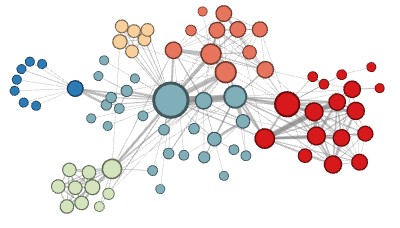
\includegraphics[width=0.85\linewidth]{homo.png}
  \caption{The Color coded communities exhibiting homophily discovered by node2vec in the Les Misérables Network \cite{node2vec-kdd2016}}
  \label{fig:boat1}
\end{figure}

\section{Related Works}

This benchmarking assignment is being undertaken by 4 other groups of students, working on different models such as Struct2vec (\cite{ribeiro2017struc2vec}), Position Aware GNNs (\cite{you2019position}),  Graph Attention Networks (\cite{velivckovic2017graph}), Graph Convolutional Networks (\cite{kipf2016semi}) and GraphSage (\cite{hamilton2017inductive}). \\
Additionally, \citet{dwivedi2020benchmarking} provides a framework for benchmarking GNNs.

\newpage
\section{Datasets}

\begin{table}[b!]
\begin{center}
\begin{tabular}{ c|c|c|c } 
%  \hline
  & \textbf{Protein} & \textbf{PPI} & \textbf{Brightkite}  \\ 
 \hline
\textbf{\# Nodes} & 43,471 & 56,944 & 58,228\\ 
%  \hline
\textbf{\# Edges} & 162,088 & 818,716 & 214,078 \\
%  \hline
\textbf{\# Classes} & 3 & 121 (Multilabel) & - \\
%  \hline
\textbf{\# Features} & 29 & 50 & - \\
%  \hline
\textbf{ Task} & I & II, III & II \\
%  \hline
\end{tabular}
\end{center}
\caption{\textmd{Summary of the datasets used in our experiments}}
\label{tab:tab1}
\end{table}

We used the following 3 datasets for benchmarking:
\begin{center}
\begin{tabular}{l l}
\textbf{Protein} & (\citet{10.1093/bioinformatics/bti1007})\\
\textbf{Protein Protein Interaction (PPI)} & (\citet{Zitnik2017}) \\
\textbf{Brightkite} & (\citet{cho2011friendship})
\end{tabular}
\end{center}
  
\subsection{PPI}

24 Protein-protein interaction networks from \citet{Zitnik2017}. Each graph has 3000 nodes with avg. degree 28.8, each node has 50 dimensional feature vector.  Protein-protein interactions (PPIs) are essential to almost every process in a cell, so understanding PPIs is crucial for understanding cell physiology in normal and disease states. It is also essential in drug development, since drugs can affect PPIs. Protein-protein interaction networks (PPIN) are mathematical representations of the physical contacts between proteins in the cell. \\
We use the this dataset for the multilabel node classification task and the link prediction task.

\subsection{Protein}

1113 protein graphs from \citet{10.1093/bioinformatics/bti1007}. Each node is labeled with a functional role of the protein. Each node has a 29 dimensional feature vector. \\
We use the this dataset for the pairwise node classification task

\subsection{Brightkite}

Brightkite from \citet{cho2011friendship} was once a location-based social networking service provider where users shared their locations by checking-in. The friendship network was collected using their public API, and consists of 58,228 nodes and 214,078 edges. The network is originally directed but they have constructed a network with undirected edges when there is a friendship in both ways. We have also collected a total of 4,491,143 check-ins of these users over the period of Apr. 2008 - Oct. 2010 \\
We use the this dataset for the link prediction task.

\section{Prediction Tasks}
In this section, we describe in detail the benchmark prediction tasks that we have carried out, as well as the generation of the task-specific dataset.


\subsection{Pair-wise node classification}
Given two nodes, predict if they belong to the same class. This task aims to showcase the similarity of node features/neighbourhoods which influence the class of the node.\\

We have used the Protein \cite{10.1093/bioinformatics/bti1007} dataset for this task. Our total dataset size was 400,000, which was split for 5-fold cross validation. This was generated by random node-pair sampling equally from the positive samples (both nodes have same class label) and negative samples. The weightage of each class (Class 0, Class 1 \& Class 2) was proportionate to the number of nodes in that class.


\subsection{Link Prediction}
To predict if there is an edge between two nodes. In link prediction tasks two nodes are generally more likely to form a link, if they are close together in the graph. \\
We have used the PPI dataset \cite{Zitnik2017} and the Brightkite dataset \cite{cho2011friendship} for this task. Our total dataset size was 2 times the number of edges in the respective datasets. The negative samples were generated by random sampling of node pairs which don't have edges between them. 

\subsection{Multi-class node classification}
To predict the class labels for a given node. For the multi-class/ multi-label setting, each node has an associated class label vector. \\
We have used the PPI dataset \cite{Zitnik2017} for this task. Each node had an associated 121-dimension binary class label vector, where multiple values can be 1. On average, a node has ~37 class labels active (Range 0-101).


\section{Experimental Setup}

In this section we outline the scoring methods, implementation details, aggregating functions for both our models and tasks.

\subsection{Scoring Methods}
\textbf{ROC AUC:} Area Under the Receiver Operating Characteristic Curve (ROC AUC) from prediction scores.  It tells how much model is capable of distinguishing between classes. Higher the AUC, better the model is at predicting 0s as 0s and 1s as 1s.
\\
\textbf{Precision:} It is the ratio TP / (TP + FP) where TP is the number of true positives and FP the number of false positives. The precision is intuitively the ability of the classifier for successful prediction. The best value is 1 and the worst value is 0.
\\
\textbf{Recall:} It is the ratio TP / (TP + FN) where TP is the number of true positives and FN the number of false negatives. The recall is intuitively the ability of the classifier to find all the positive samples. The best value is 1 and the worst value is 0.
\\
\textbf{F1 score:} By itself, neither Precision nor Recall are able to capture the classifiers complete performance. So, the F1 score is used to convey the balance between the precision and recall. It is the harmonic mean of Precision and Recall. 

\subsection{DeepWalk}

DeepWalk by \citet{Perozzi:2014:DOL:2623330.2623732} is an algorithm that is used to create embeddings of the nodes in a graph. The embeddings are meant to encode the community structure of the graph. It achieves this by using SkipGram to create the embeddings.
\\
The method used to make predictions is skip-gram, just like in Word2vec architecture for text. Instead of running along the text corpus, DeepWalk runs along the graph to learn an embedding. The model can take a target node to predict it’s “context”, which in the case of a graph, means it’s connectivity, structural role, and node features.
\\
Although DeepWalk is relatively efficient with a score of \textbf{$O(|V|)$}, this approach is transductive, meaning whenever a new node is added, the model must be retrained to embed and learn from the new node.

\subsection{Node2vec}

Node2vec by \citet{node2vec-kdd2016} is an algorithmic framework for representational learning on graphs. Given any graph, it can learn continuous feature representations for the nodes, which can then be used for various downstream machine learning tasks. \\
The node2vec framework learns low-dimensional representations for nodes in a graph by optimizing a neighborhood preserving objective. The objective is flexible, and the algorithm accommodates for various definitions of network neighborhoods by simulating biased random walks. Specifically, it provides a way of balancing the exploration-exploitation tradeoff that in turn leads to representations obeying a spectrum of equivalences from homophily to structural equivalence.

\subsection{Differences}

The difference between Node2vec and DeepWalk is subtle but significant. Node2vec features a walk bias variable $\alpha$, which is parameterized by $p$ and $p$. The parameter $p$ prioritizes a breadth-first-search (BFS) procedure, while the parameter $p$ prioritizes a depth-first-search (DFS) procedure. The decision of where to walk next is therefore influenced by probabilities $\frac{1}{p}$ or $\frac{1}{q}$. \\

BFS is ideal for learning local neighbors, while DFS is better for learning global variables. Node2vec can switch to and from the two priorities depending on the task. This means that given a single graph, Node2vec can return different results depending on the values of the parameters. As per DeepWalk, Node2vec also takes the latent embedding of the walks and uses them as input to a neural network to classify nodes. \\

Experiments demonstrated that BFS is better at classifying according to structural roles (hubs, bridges, outliers, etc.) while DFS returns a more community driven classification scheme.

\subsection{Implementation details}

\begin{table}[h]
\begin{center}
\begin{tabular}{ c|c|c } 
%  \hline
 \textbf{Parameters} & \textbf{Range} & \textbf{Default Value} \\ 
 \hline
 No. of walks & 10,30,100,300 & 10 \\
%  \hline
 Embedding size & 32,64,128,256 & 128 \\ 
%  \hline
 Walk Length & 5,15,50,80,100 & 80 \\ 
%  \hline
 Window size - Skipgram & 5,10,20 & 10 \\ 
%  \hline
 Iters of SGD & 1,5,10,50,100 & 1 \\ 
%  \hline
 Return hyperparameter & 0.1,0.5,1,2,10 & 1 \\ 
%  \hline
 Inout hyperparameter & 0.1,0.5,1,2,10 & 1 \\ 
%  \hline
\end{tabular}
\end{center}
\caption{Paramters variation for Node2vec}
\label{tab:node2vec_param}
\end{table}

\begin{table}[h]
\begin{center}
\begin{tabular}{ c|c|c } 
%  \hline
 \textbf{Parameters} & \textbf{Range} & \textbf{Default} \\ 
 \hline
 No. of walk & 10,30,100,300 & 10 \\
%  \hline
 Embedding size & 32,64,128,256 & 64 \\ 
%  \hline
 Walk Length & 5,15,50,100 & 40 \\ 
%  \hline
 Window size for Skipgram & 5,10,20 & 5 \\ 
%  \hline

\end{tabular}
\end{center}
\caption{Paramters variation for DeepWalk}
\label{tab:deepwalk_param}
\end{table}

We use the standard node2vec implementation available at \href{https://github.com/aditya-grover/node2vec}{github.com/aditya-grover/node2vec}, implemented in Python2.7 and the standard DeepWalk implementation available at \href{https://github.com/phanein/deepwalk}{github.com/phanein/deepwalk}, implemented in Python3.7 \\

We perform extensive hyperparameter tuning to decide the optimal parameters for this model. A summary of the parameters used are summarised in Table \ref{tab:node2vec_param} and Table \ref{tab:deepwalk_param}. \\

\begin{table}[h]
\begin{center}
\begin{tabular}{ c|c|c } 
%  \hline
 \textbf{Operator} & \textbf{Symbol} & \textbf{Definition} \\ 
 \hline
 Average & $\boxplus$ & $\frac{f_{i}(u) + f_{i}(v)}{2}$ \\
%  \hline
 Hadamard & $\boxdot$ & $f_{i}(u) * f_{i}(v)$ \\ 
%  \hline
 Weighted-L1 & $\vert\vert \cdot \vert\vert_{\bar{1}}$ & $\vert f_{i}(u) - f_{i}(v) \vert$ \\ 
%  \hline
 Weighted-L2 & $\vert\vert \cdot \vert\vert_{\bar{2}}$ & $\vert f_{i}(u) - f_{i}(v) \vert^{2}$ \\ 
%  \hline

\end{tabular}
\end{center}
\caption{Choice of operators for learning edge features}
\label{tab:agg}
\end{table}

For Task I (Pairwise Node Classification) and Task II (Link Prediction), as per \cite{node2vec-kdd2016} we try out 4 aggregator functions shown in Table \ref{tab:agg} to join the embeddings of the two nodes and these are passed to a secondary classifier (using Logistic Regression as per \cite{node2vec-kdd2016}). \\
For Task III (Multi-Label Classification) we train multiple one-vs-rest logistic regression classifiers (as per \cite{node2vec-kdd2016}). \\
Additionally, we experiment with various other classifiers (Linear SVM Classifier, Extra Trees Classifier, Bagging Classifier, Gradient Boosting Classifier, AdaBoost Classifier and MLP Classifier). For all of them we use the sklearn-implementation.  
\newpage
\section{Results}

All results are averaged over 5-fold cross validation. The training specifications are as per those mentioned previously.

\subsection{Pair-wise node classification}

\begin{table}[h]
\begin{center}
\begin{tabular}{ c|c|c|c|c|c } 
 \textbf{Network} & \textbf{Dataset} & \textbf{ROC} & \textbf{Precision} & \textbf{Recall} & \textbf{$F_{1}$} \\ 
 \hline
 GCN\cite{kipf2016semi} & Protein &  0.515 & - & - & - \\
 GraphSAGE\cite{hamilton2017inductive} & Protein & 0.520 & - & - & - \\
 GAT\cite{velivckovic2017graph} & Protein &  0.528 & - & - & - \\
 GIN\cite{wang2019knowledge} & Protein & 0.523 & - & - & - \\
 P-GNN\cite{you2019position} & Protein & \textbf{0.729} & - & - & - \\
 \hline
 Node2Vec\cite{node2vec-kdd2016} & Protein & 0.604 & 0.600 & 0.625 & 0.612  \\ 
 Deepwalk\cite{Perozzi:2014:DOL:2623330.2623732} & Protein & 0.557 & 0.555 & 0.567 & 0.561

\end{tabular}
\end{center}
\caption{Pairwise Node Classification on Protein Dataset}
\label{tab:res1}
\end{table}

Node2vec outperforms Deepwalk, and they both outperform other networks such as GCN, GraphSAGE, GAT, GIN etc. \\
However, this may be due to these networks performing this task in the inductive setting whereas Node2vec and Deepwalk use the transductive setting. \\
Hence, since no node/graph is technically "unseen", they can perform better than the indcutive setting algorithms


\subsection{Link Prediction}

\begin{table}[h]
\begin{center}
\begin{tabular}{ c|c|c|c|c|c } 
\textbf{Network} & \textbf{Dataset} & \textbf{ROC} & \textbf{Precision} & \textbf{Recall} & \textbf{$F_{1}$} \\ 
 \hline
 GCN\cite{kipf2016semi} & PPI &  0.769 & - & - & - \\
 GraphSAGE\cite{hamilton2017inductive} & PPI & 0.803 & - & - & - \\
 GAT\cite{velivckovic2017graph} & PPI &  0.783 & - & - & - \\
 GIN\cite{wang2019knowledge} & PPI & 0.782 & - & - & - \\
 P-GNN\cite{you2019position} & PPI & \textbf{0.808} & - & - & - \\
 \hline
 Node2Vec\cite{node2vec-kdd2016} & PPI & 0.557 & 0.557 & 0.559 & 0.558  \\ 
 Deepwalk\cite{Perozzi:2014:DOL:2623330.2623732} & PPI & 0.553 & 0.549 & 0.596 & 0.571  \\
 \hline
 \hline
 Node2Vec\cite{node2vec-kdd2016} & BrightKite & \textbf{0.813} & 0.844 & 0.769 & 0.804  \\ 
 Deepwalk\cite{Perozzi:2014:DOL:2623330.2623732} & BrightKite & 0.742 & 0.728 & 0.773 & 0.750

\end{tabular}
\end{center}
\caption{Link Prediction on PPI and Brightkite Dataset}
\label{tab:res2}
\end{table}

Node2vec outperforms Deepwalk, however they are both beaten by other networks such as GCN, GraphSAGE, GAT, GIN, P-GNN etc. \\
This may be due to the fact that Node2vec and DeepWalk don't use any node features during their training, and rely only on the neighbourhood of the node

\subsection{Multi-Label Node Classification}

\begin{table}[h]
\begin{center}
\begin{tabular}{ c|c|c|c|c|c } 
 \textbf{Network} & \textbf{Dataset} & \textbf{Precision} & \textbf{Recall} & \textbf{Micro $F_{1}$} \\ 
 \hline
 Random & PPI & - & - & 0.396 \\
 MLP & PPI & - & - & 0.422 \\
 GraphSAGE\cite{hamilton2017inductive} & PPI & - & - & 0.768 \\
 GAT\cite{velivckovic2017graph} & PPI & - & - & 0.973 \\
 \hline
 Node2Vec\cite{node2vec-kdd2016} & PPI & 0.419 & 0.609 & 0.479  \\ 
 Deepwalk\cite{Perozzi:2014:DOL:2623330.2623732} & PPI & 0.363 & 0.594 & 0.431

\end{tabular}
\end{center}
\caption{Node Classification on PPI Dataset}
\label{tab:res3}
\end{table}

Node2vec outperforms Deepwalk, however they are both beaten by other networks such as GraphSAGE, GAT etc. \\
Since PPI has over 121 distinct labels per node, it is difficult to predict each and every one of them accurately with only the neighbourhood information of the node \\
\newpage

\section{Variations and Improvements}
This section serves to highlight certain experiments and variations to the models and parameters done by us.
\subsection{Classifiers}

Apart from the standard logistic regression classifier mentioned in the papers, we experimented with a couple of other classifiers and ensembles. RandomForests with 100 trees gives us the best results for both methods.

\begin{table}[h]
\begin{center}
\begin{tabular}{ c|c|c|c|c|c|c } 
\textbf{Network} & \textbf{Classifier} & \textbf{ROC} & \textbf{Precision} & \textbf{Recall} & \textbf{$F_{1}$} \\ 
\hline
& Logistic & 0.604 & 0.6 & 0.625 & 0.612 \\
& LinearSVC & 0.604 & 0.6 & 0.626 & 0.612 \\
& ExtraTrees & 0.625 & 0.619 & 0.65 & 0.634 \\
Node2vec & Bagging & 0.559 & 0.575 & 0.455 & 0.508 \\
& RandomForest & \textbf{0.626} & 0.62 & 0.654 & 0.636 \\
& GradientBoost & 0.612 & 0.602 & 0.661 & 0.63 \\
& AdaBoost & 0.57 & 0.568 & 0.582 & 0.575 \\
\hline
& Logistic & 0.557 & 0.555 & 0.567 & 0.561 \\
& LinearSVC & 0.557 & 0.556 & 0.568 & 0.562 \\
& ExtraTrees & 0.575 & 0.579 & 0.546 & 0.562 \\
Deepwalk & Bagging & 0.536 & 0.548 & 0.418 & 0.474 \\
& RandomForest & \textbf{0.577} & 0.579 & 0.562 & 0.57 \\
& GradientBoost & 0.561 & 0.559 & 0.577 & 0.568 \\
& AdaBoost & 0.537 & 0.537 & 0.537 & 0.537
\end{tabular}
\end{center}
\caption{Variation across Classifiers for Task I}
\label{tab:res4.2}
\end{table}

\subsection{Aggregator Functions}
The Average binary operator performs the best among the four aggregator functions. This might be since the Hadamard operator supresses a dimension even if one operand is zero in the same, and the L1 and L2 values capture only the relative distance between the operands however are unable to incorporate the position of the operands in a global coordinate.

\begin{table}[h]
\begin{center}
\begin{tabular}{ c|c|c|c|c|c|c } 
\textbf{Network} & \textbf{Operator} & \textbf{ROC} & \textbf{Precision} & \textbf{Recall} & \textbf{$F_{1}$} \\ 
\hline
& Average & \textbf{0.604} & 0.600 & 0.625 & 0.612  \\ 
Node2Vec & Hadamard & 0.561 & 0.561 & 0.566 & 563  \\ 
& Weighted-L1 & 0.555 & 0.555 & 0.563 & 0.559  \\ 
& Weighted-L2 & 0.557 & 0.556 & 0.567 & 0.561  \\ 
\hline
& Average & \textbf{0.557} & 0.555 & 0.567 & 0.561x  \\
Deepwalk& Hadamard &  0.517 & 0.517 & 0.516 & 0.516  \\
& Weighted-L1 & 0.531 & 0.531 & 0.530 & 0.530  \\
& Weighted-L2 & 0.531 & 0.531 & 0.533 & 0.532
\end{tabular}
\end{center}
\caption{Variation across Binary Aggregator Functions for Task I}
\label{tab:res4.1}
\end{table}
\newpage

\subsection{Parameters}
This section contains a variation analysis of both methods varying some common hyper-parameters of the models for Task I. \\

\begin{figure}[h]
  \centering
  \begin{subfigure}[b]{0.49\linewidth}
    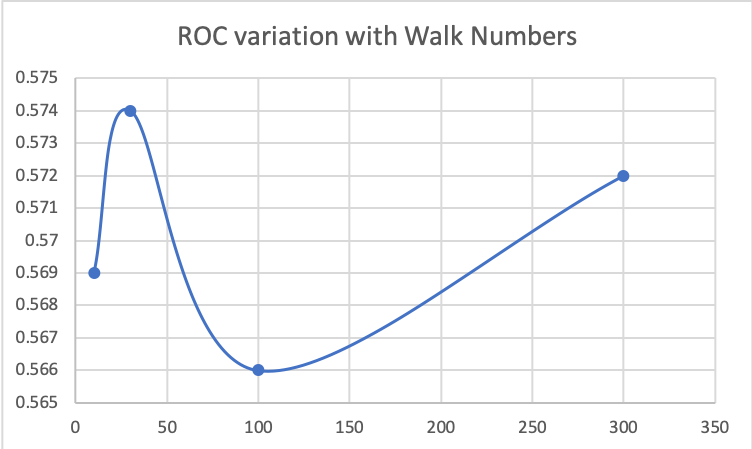
\includegraphics[width=\linewidth]{Images/Picture 1.png}
    \caption{Walk Numbers}
  \end{subfigure}
  \begin{subfigure}[b]{0.49\linewidth}
    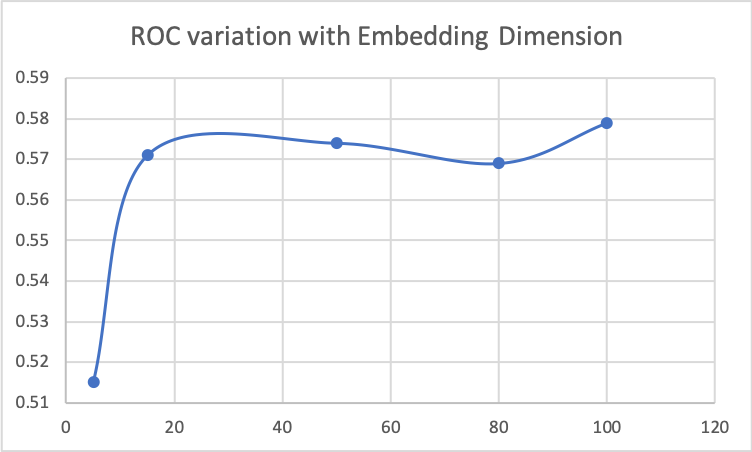
\includegraphics[width=\linewidth]{Images/Picture 2.png}
    \caption{Embedding Dimensions}
  \end{subfigure}
  \begin{subfigure}[b]{0.49\linewidth}
    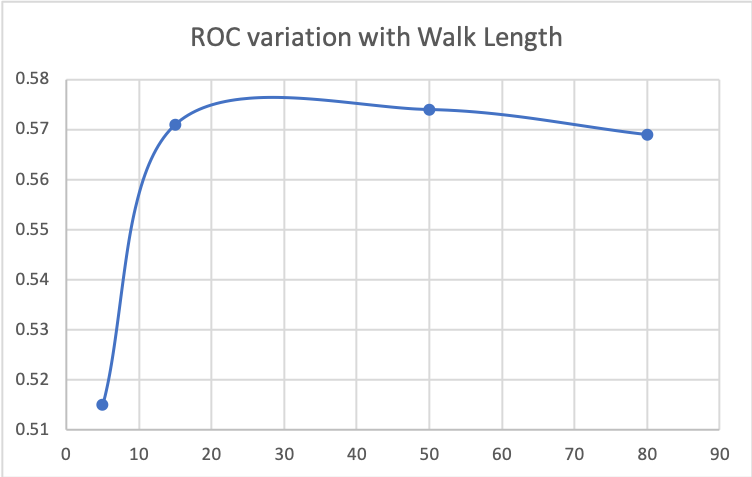
\includegraphics[width=\linewidth]{Images/Picture 3.png}
    \caption{Walk Length}
  \end{subfigure}
  \begin{subfigure}[b]{0.49\linewidth}
    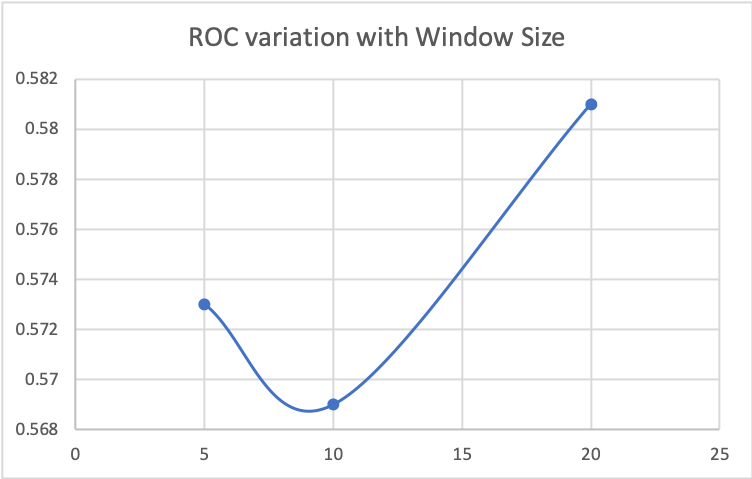
\includegraphics[width=\linewidth]{Images/Picture 4.png}
    \caption{Window Size}
  \end{subfigure}
  \begin{subfigure}[b]{0.49\linewidth}
    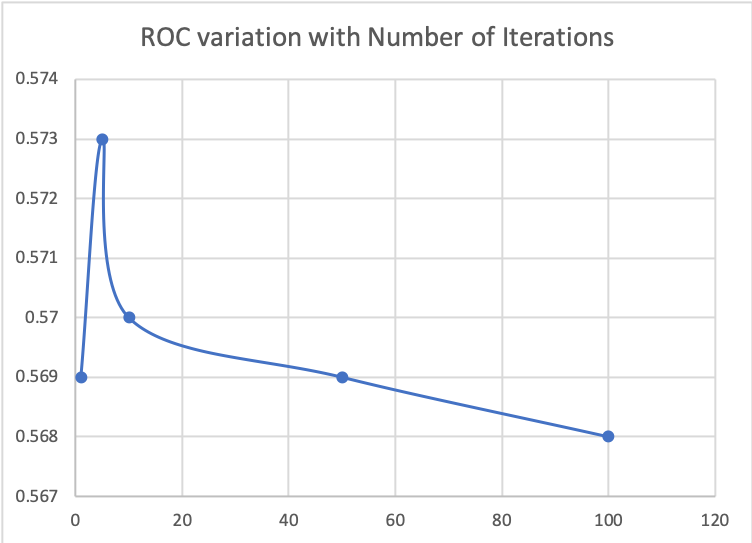
\includegraphics[width=\linewidth]{Images/Picture 5.png}
    \caption{Iterations}
  \end{subfigure}
  \begin{subfigure}[b]{0.49\linewidth}
    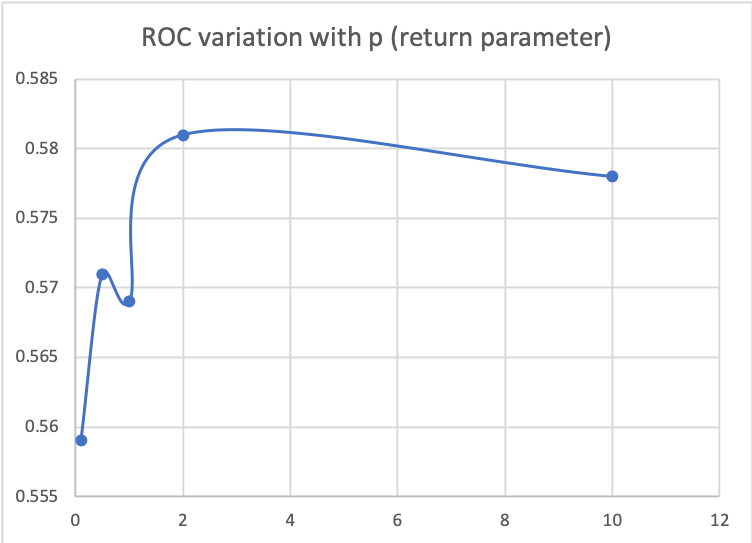
\includegraphics[width=\linewidth]{Images/Picture 6.png}
    \caption{Return Parameter}
  \end{subfigure}
  \begin{subfigure}[b]{0.49\linewidth}
    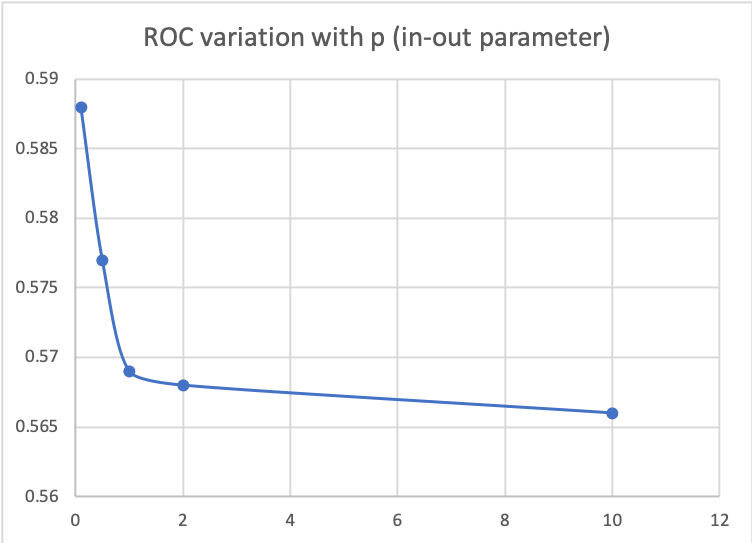
\includegraphics[width=\linewidth]{Images/Picture 7.png}
    \caption{In-Out Parameter}
  \end{subfigure}
  \caption{The results for Parameter Variation on Node2vec}
  \label{fig:res4.3}
\end{figure}

\begin{figure}[h]
  \centering
  \begin{subfigure}[b]{0.49\linewidth}
    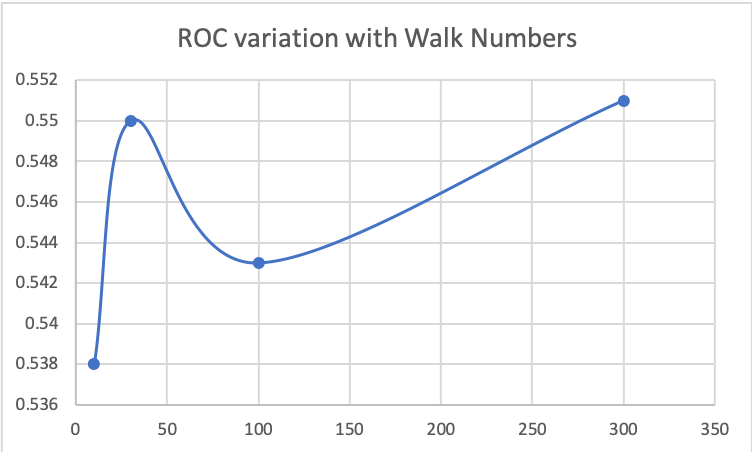
\includegraphics[width=\linewidth]{Images/Picture 1.1.png}
    \caption{Walk Numbers}
  \end{subfigure}
  \begin{subfigure}[b]{0.49\linewidth}
    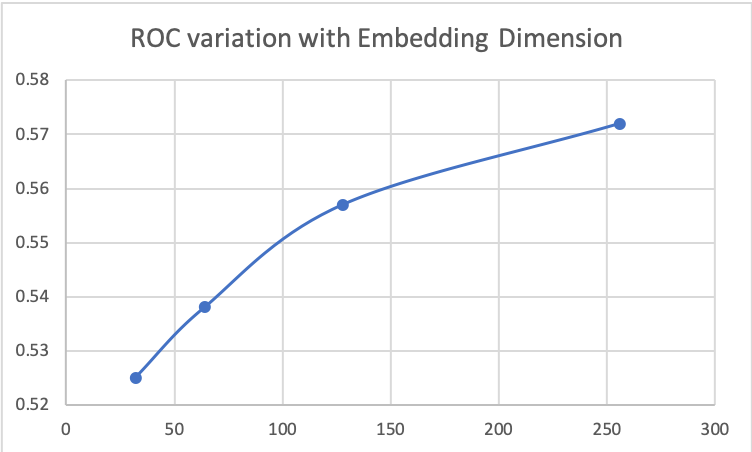
\includegraphics[width=\linewidth]{Images/Picture 1.2.png}
    \caption{Embedding Dimensions}
  \end{subfigure}
  \begin{subfigure}[b]{0.49\linewidth}
    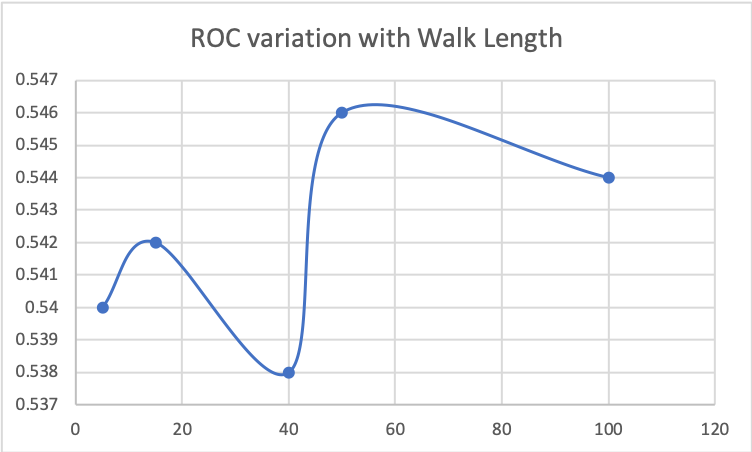
\includegraphics[width=\linewidth]{Images/Picture 1.3.png}
    \caption{Walk Length}
  \end{subfigure}
  \begin{subfigure}[b]{0.49\linewidth}
    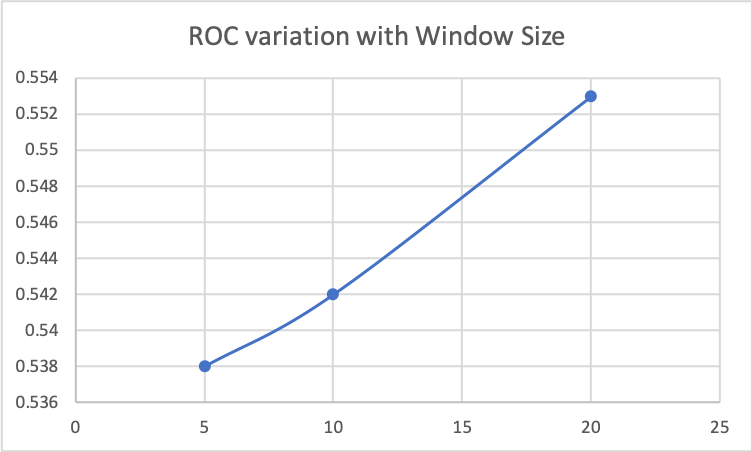
\includegraphics[width=\linewidth]{Images/Picture 1.4.png}
    \caption{Window Size}
  \end{subfigure}
  \caption{The results for Parameter Variation on DeepWalk}
  \label{fig:res4.4}
\end{figure}


%%
%% The acknowledgments section is defined using the "acks" environment
%% (and NOT an unnumbered section). This ensures the proper
%% identification of the section in the article metadata, and the
%% consistent spelling of the heading.
\newpage
\section{Conclusion}
From this benchmarking excercise, we observe Node2vec has an improvement over DeepWalk in all 3 tasks, i.e., Pairwise Node Classification, Link Predicion and Multi-Label Node Classification. This is since Node2vec looks at both local and global neighbourhoods through it's combination of BFS and DFS. It is therefore able to learn a better context for the node as compared to Deepwalk. \\
We also would like to point out that DeepWalk was released in 2014, and Node2vec in 2016. Moreover, since then there have been some significant improvements in GNNs which have vastly improved the results on these three tasks.

\newpage
%%
%% The next two lines define the bibliography style to be used, and
%% the bibliography file.
\bibliographystyle{ACM-Reference-Format}
\bibliography{sample-base}

%%
%% If your work has an appendix, this is the place to put it.
% \appendix

% \section{Research Methods}

% \subsection{Part One}

% Lorem ipsum dolor sit amet, consectetur adipiscing elit. Morbi
% malesuada, quam in pulvinar varius, metus nunc fermentum urna, id
% sollicitudin purus odio sit amet enim. Aliquam ullamcorper eu ipsum
% vel mollis. Curabitur quis dictum nisl. Phasellus vel semper risus, et
% lacinia dolor. Integer ultricies commodo sem nec semper.

% \subsection{Part Two}

% Etiam commodo feugiat nisl pulvinar pellentesque. Etiam auctor sodales
% ligula, non varius nibh pulvinar semper. Suspendisse nec lectus non
% ipsum convallis congue hendrerit vitae sapien. Donec at laoreet
% eros. Vivamus non purus placerat, scelerisque diam eu, cursus
% ante. Etiam aliquam tortor auctor efficitur mattis.

% \section{Online Resources}

% Nam id fermentum dui. Suspendisse sagittis tortor a nulla mollis, in
% pulvinar ex pretium. Sed interdum orci quis metus euismod, et sagittis
% enim maximus. Vestibulum gravida massa ut felis suscipit
% congue. Quisque mattis elit a risus ultrices commodo venenatis eget
% dui. Etiam sagittis eleifend elementum.

% Nam interdum magna at lectus dignissim, ac dignissim lorem
% rhoncus. Maecenas eu arcu ac neque placerat aliquam. Nunc pulvinar
% massa et mattis lacinia.

\end{document}
\endinput
%%
%% End of file `sample-sigconf.tex'.
